\documentclass[12pt]{article}
\usepackage[utf8]{inputenc}
\usepackage[T2A]{fontenc}
\usepackage[russian]{babel}
\usepackage{amsmath}
\usepackage{amssymb}
\usepackage{dsfont}
\usepackage[dvipsnames]{xcolor}
\usepackage{setspace}
\usepackage{multirow}
\usepackage[a4paper, outer=1.5cm, inner=1.5cm, top=1cm, bottom=1cm]{geometry}
\usepackage{graphicx}
\usepackage{skull}
\usepackage{wasysym}
\usepackage{float}
\graphicspath{{.images/}}
\usepackage{hyperref}
\hypersetup{colorlinks=true, linkcolor=blue, filecolor=magenta, urlcolor=cyan}
\usepackage[firstpage]{draftwatermark}
\SetWatermarkText{
    $\qquad\qquad\qquad\qquad\qquad$\parbox{7cm}{\begin{center}
    
\includegraphics[width = 0.08\textwidth]{lion-logo.png}\bigskip\\~\bigskip\\~\vspace{-24mm}\\~\end{center}}
}
\SetWatermarkAngle{0}
\SetWatermarkScale{1.5}
\usepackage{etoolbox}

\newtoggle{ifsolved}
\newtoggle{needhelp}
\newcounter{num}
\setcounter{num}{1}

\newcommand{\newnum}{\par\textbf{\textnumero\arabic{num}}\stepcounter{num}}
\newcommand{\sol}{\vspace{3mm}\par\textbf{Решение: }}
\newcommand{\ans}{\vspace{3mm}\par\textbf{Ответ: }}
\newcommand{\hint}{\vspace{3mm}\par\textbf{Подсказка: }}
\newcommand{\mode}[1]{
\ifstrequal{#1}{0}{\togglefalse{ifsolved}\togglefalse{needhelp}}{\ifstrequal{#1}{1}{\togglefalse{ifsolved}\toggletrue{needhelp}}{\ifstrequal{#1}{2}{\toggletrue{ifsolved}\togglefalse{needhelp}}{\toggletrue{ifsolved}\toggletrue{needhelp}}}}} %if 0 - if 1 - if 2 - else
%\newenvironment{problem}[8]{%#1, #2, #3
%\parbox{\linewidth}{\vspace{4mm}\ifstrequal{#4}{(лёгкая)}{\newnum\textbf{.}}{\newnum\textbf{*.} } \\ #5}
%\iftoggle{ifsolved}{\sol #6}{}
%\iftoggle{ifsolved}{\ans #7}{}
%\iftoggle{needhelp}{\hint #8}{}}

\newenvironment{problem}[8]{%#1, #2, #3
\parbox{\linewidth}{\vspace{5mm}\ifstrequal{#4}{(лёгкая)}{\newnum\textbf{.}}{\newnum\textbf{*.} } \\ #5}
\iftoggle{ifsolved}{\sol #6}{}

\iftoggle{ifsolved}{\parbox{\linewidth}{\ans #7}}{}
\iftoggle{needhelp}{\parbox{\linewidth}{\hint #8}}{}}

\newenvironment{mylist} %custom list
{ \begin{itemize}
    \setlength{\itemsep}{0pt}
    \setlength{\parskip}{0pt}
    \setlength{\parsep}{0pt}     }
{ \end{itemize}                  }

\newenvironment{homeass}[1]{\vspace*{-1.5cm}
\iftoggle{ifsolved}{
    \section*{\center{Решение домашнего задания к #1.}}
}{
    \section*{\center{\textcolor{Sepia}{Домашнее задание к #1}}}
} \vspace{7mm}\large}

\parindent=0pt
\pagestyle{empty}
%$\!$[\arabic{class}.\arabic{num}]
%\ifnumcomp{\value{counter}}{>}{1}{true}{false}
%\definecolor{Gray}{gray}{0.9}
%\definecolor{mypink}{RGB}{219, 48, 122}
%\newcolumntype{g}{>{\columncolor{Gray}}p{2.8cm}}

\begin{document}
\large
\mode{7}
%0 for problems without hints
%1 for problems + hints
%2 for problems + solutions + answers
%else: show all

{\centering\section*{СПИСОК ЗАДАЧ}}

{\centering\subsection*{\smallskip\\\textcolor{green}{\textbf{Полезные вещи, которые можно и нужно копипастить:}}}}

\subsection*{\textcolor{Emerald}{\textbf{Полезные шпаргалки по LaTeXу:}}}

\textbf{Пример вставки рисунка:}

\begin{minipage}{\linewidth}
    \begin{minipage}{0.54\linewidth}
    см. рисунок справа\\
    Текст к собственно пикче, примерно всегда это либо развёрнутое описание, либо большая часть решения задачи --- стремимся экономить пространство, если это можно сделать.
    \end{minipage}
    \hspace{0.05\linewidth}
    \begin{minipage}{0.4\linewidth}
    \begin{figure}[H] 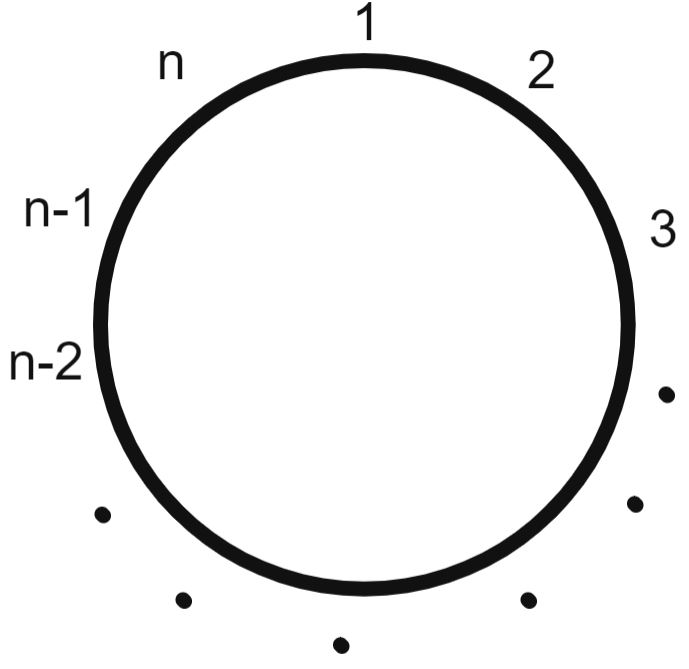
\includegraphics[width=\linewidth]{sol3} %тут поменять имя пикчи
    \end{figure}
    \end{minipage}
\end{minipage}

\textbf{Дефолтные математические знаки и символы:}\\
$\geqslant$,
$\leqslant$,
$a^{b}$,
$x_{i}$,
$\sqrt{a}$,
$\frac{a}{b}$,
$\displaystyle \frac{a}{b}$,
$\cdot$
$\;\Rightarrow\;$,
$\;\Leftrightarrow\;$,
$1{,}2$.
О промежутках:
$a\!b$,
$a\,b$,
$a\:b$,
$a\;b$,
$a\quad b$.

\textbf{Стандартные система и совокупность уравнений / неравенств:}\\
$\left\{
\begin{aligned}
f(x) &= 0 \\
g(x) &= 1
\end{aligned}\right.$

$\left[\begin{aligned}
&\left\{\begin{aligned}
f(x) &\geqslant a \\
g(x) &= b
\end{aligned}\right.\\
&\left\{\begin{aligned}
f(x) &< a \\
g(x) &= -b
\end{aligned}\right.
\end{aligned}\right.$

\subsection*{\textcolor{Emerald}{\textbf{Не математическое, но полезное:}}}
% комментарий в любом месте документа, который нигде не будет видно. Можно использовать для написания заметок-вопросов по задачам
\textbf{Пример таблицы:}

\begin{tabular}{|c|c|c|}
\hline
    $a$ & $b$ & текст
\\\hline
    $c$ & $d$ & мораль
\\\hline
\end{tabular}\\

\textbf{Отступы:} между\smallskip\\ строками\medskip\\ \textbf{Тире} --- это три дефиса.\\
\textbf{Списки:}
\begin{mylist}
\item [$\bullet$] это был пункт а
\item [2)] а это уже пункт номер 2 с изменённым заголовком
\end{mylist}

\subsection*{\textcolor{Emerald}{\textbf{Всё, неупомянутое выше (или если просто что-то не так):}}}
\begin{mylist}
\item [$\bullet$] Решение отдельных вопросов касательно ТеХа нужно искать в \href{https://www.mccme.ru/free-books/llang/newllang.pdf}{Львовском}.

\item [$\bullet$] Найти произвольный символ, который нужен, можно в \href{http://detexify.kirelabs.org/classify.html}{Detexify}.

\item [$\bullet$] Если возникли сомнения при решении, ответ практически ко всем задачам можно проверить с помощью \href{https://www.wolframalpha.com/}{WolframAlpha}.

\item [$\bullet$] Если в задаче нужно создать картинку, то лучше пока отложить эту задачу. Все графики планируется централизованно нарисовать (или перерисовать) в геогебре.

\item [\textcolor{brown}{\textbf{!!}}] Важно ставить \textcolor{red}{\textbf{$\spadesuit$}}
(или просто red) в тело задачи в случае серьёзных вопросов к решению и какой-то вопиющей лажи.

\item [\textcolor{brown}{\textbf{!!}}] Важно ставить \textcolor{olive}{\textbf{$\spadesuit$}}
(или просто olive) в тело задачи в случае не самого удачного текста и кривых отступов.
\end{mylist}

\subsection*{\textcolor{Violet}{\textbf{Комментарии:}}}% а также невидимые комментарии - так можно оставлять заметки-вопросы прямо в задаче, чтобы потом было понятно, в чём вопрос.
\begin{mylist}
\item [$\skull$] Переставлять задачи местами --- очень плохая идея.

\item [$\smiley$] При двойном клике по тексту pdf справа происходит автоматический переход к этому месту в латех-коде, а для обратного перехода можно нажать стрелку вправо (висит сверху между pdf и латех-кодом).

\item [$\smiley$] Если есть размышления, дописывать red/olive к задаче или не дописывать, то лучше всё-таки дописать.

\item [$\skull$] Самое плохое, что можно сделать --- написать в любое поле из трёх (НаписанноеРешение/ВерныйОтвет/Подсказка) только половину того, что надо, никак это не отметить, и потом пойти дальше.\\ Нужно в этот момент писать red/olive в случайном месте задачи, чтобы потом вычислить это с помощью Ctrl+F по всему документу (и это то, что потом будет делаться долго и тщательно)
\end{mylist}

\newpage
\setcounter{num}{278}

\hypertarget{6.7}{{\centering\section*{\bigskip\\\textcolor{Blue}{\hyperlink{start2}{\textcolor{Blue}{6.7}} Рациональные числа.}\vspace{-5mm}}}}

\begin{problem}{Сложение чисел с любыми знаками.}{6.7.2}{Киселёв}{(лёгкая)}
{Ресторан получил прибыль: в январе $a$ рублей и в феврале $b$ рублей.\\ Сколько прибыли получил ресторан за два месяца?}
{НаписанноеРешение}
{ВерныйОтвет}{Подсказка}
\end{problem}

\begin{problem}{Сложение чисел с любыми знаками.}{6.7.2}{Киселёв}{(лёгкая)}
{Температура на улице 18-ого января составляла $-21^\circ$С. Через два дня температура поднялась на 12 градусов. Какая была температура на улице 20-ого января?}
{НаписанноеРешение}
{ВерныйОтвет}{Подсказка}
\end{problem}

\begin{problem}{Вычитание.}{6.7.3}{Киселёв}{(лёгкая)}
{Прибыль фабрики за 2 месяца, январь и февраль, составила $a$ рублей. Как велика была прибыль за один февраль, если известно, что за январь фабрика дала $b$ рублей прибыли?}
{НаписанноеРешение}
{ВерныйОтвет}{Подсказка}
\end{problem}

\begin{problem}{Вычитание.}{6.7.3}{Киселёв}{(лёгкая)}
{Товар купили за $a$ рублей, а продали за $b$ рублей. Сколько получено прибыли? Вычислить эту прибыль, если $a = 40$ и $b = 35$. Что означает здесь отрицательный ответ?}
{НаписанноеРешение}
{ВерныйОтвет}{Подсказка}
\end{problem}

\begin{problem}{Вычитание.}{6.7.3}{Киселёв}{(лёгкая)}
{Некто ежемесячно получает дохода $m$ рублей, а тратит $n$ рублей. Сколько у него остаётся ежемесячно? Вычислить ответ при $m = 120000$ и $n = 130000$.\\ Что означает отрицательный ответ?}
{За месяц в итоге выйдет $120000 - 130000 = -10000$ рублей. То есть весь доход за месяц будет потрачен, а также сверх этого будут потрачены ещё 10000 рублей (возможно, они были отложены заранее). Отрицательный ответ означает, что в результате за месяц количество денег не увеличилось на 10000 рублей, а уменьшилось на 10000 рублей.}
{За месяц этот человек получает $-10000$ рублей (то есть, его состояние уменьшается на десять тысяч рублей каждый месяц).}{Найди разность.}
\end{problem}

\begin{problem}{Вычитание.}{6.7.3}{6S}{(лёгкая)}
{Впиши вместо $\ast$ числа так, чтобы каждое число, начиная с третьего (считая слева направо), равнялось сумме двух предшествующих ему чисел: $\;\ast\; \ast\; \ast \;\ast \;\ast\; \ast\; \ast \;\, 2\,\; 0 \;\ast\; \ast$

}
{НаписанноеРешение}
{ВерныйОтвет}{Подсказка}
\end{problem}

\begin{problem}{Умножение.}{6.7.4}{6S}{(лёгкая)}
{По автомобильной дороге Москва-Смоленск едет машина со средней скоростью $v$ км/ч. В полдень машина находилась около города Вязьма. Где будет находиться машина через $t$ часов? Дать точный ответ при $v = 60$, $t = 3$.}
{НаписанноеРешение}
{ВерныйОтвет}{Подсказка}
\end{problem}

\begin{problem}{Умножение.}{6.7.4}{6S}{(лёгкая)}
{По дороге из Москвы в Казань едет мотоциклист со средней скоростью $v$ км/ч.\\ В 15:00 мотоциклист проехал город Нижний Новгород. Где был этот мотоциклист $3$ часа назад, в полдень?}
{НаписанноеРешение}
{ВерныйОтвет}{Подсказка}
\end{problem}

\begin{problem}{Умножение.}{6.7.4}{6K}{(лёгкая)}
{Положительным или отрицательным является выражение $3ac - 5b$, если числа $a$, $b$, $c$ отрицательны?}
{Если перемножить $a$ и $c$, то так как оба числа отрицательны, в результате получится положительное число (поменяли направление два раза --- число остаётся положительным; минус на минус даёт плюс). Число $3ac = 3\cdot ac$ --- произведение двух положительных чисел, поэтому оно тоже положительно.\\ Осталось вычесть $5b$. Число $b$ отрицательно, а значит, и число в 5 раз большее, $5b$, также отрицательно. Вычесть отрицательное число --- то же, что и прибавить положительное. В итоге наше выражение --- сумма двух положительных чисел: $3ac - 5b = 3ac + ({-}5b)$, и поэтому выражение является положительным числом.}
{Если $a$, $b$, $c$ --- отрицательны, выражение $3ac - 5b$ положительно.}{Является число $ac$ положительным или отрицательным? А $3ac$?}
\end{problem}

\begin{problem}{Умножение.}{6.7.4}{6K}{(лёгкая)}
{Известно, что числа $a$ и $b$ отрицательны, а число $c$ --- положительно.\\ Является ли выражение $2 - 3a - 5bc + 8abc$ положительным или отрицательным, и если да, то почему?}
{$3a$ --- отрицательное число, так как $a$ отрицательно. $5bc$ --- произведение отрицательного и положительного чисел, а значит также отрицательно.\\ $8abc = 8\cdot ab \cdot c$ --- произведение трёх положительных чисел ($ab > 0$, ведь <<минус на минус даёт плюс>>), и потому положительно. Получается, что наше выражение это $2 - \text{отрицательное} - \text{отрицательное} + \text{положительное}$.\\ Вычитание отрицательного --- тоже самое, что и прибавление положительного, поэтому получаемый результат всегда будет положителен.}
{Это выражение всегда положительно, отрицательным оно быть не может.}{Положительны или отрицательны числа $3a$, $5bc$, $8abc$?}
\end{problem}

\begin{problem}{Умножение.}{6.7.4}{6S \textcolor{red}{\textbf{$\spadesuit$}}}{*}
{Произведение двух нечётных однозначных натуральных чисел на 7 больше их суммы. Найти эти числа.}
{НаписанноеРешение}
{ВерныйОтвет}{Подсказка}
\end{problem}

\begin{problem}{Деление.}{6.7.5}{6K}{(лёгкая)}
{Известно, что числа $p$ и $q$ положительны, а число $n$ --- отрицательно.\\ Является ли выражение $\frac{p}{q} - \frac{1}{n}$ положительным или отрицательным? Почему?}
{Дробь $\frac pq$ является положительным числом, $\frac 1n$ --- отрицательным.\\ Поэтому $\frac pq - \frac1n$ --- положительное число (вычли отрицательное).}
{Выражение $\frac pq - \frac1n$ всегда положительно.}{Положительной или отрицательной является дробь $\frac1n$?\\ Что получаем после вычитания?}
\end{problem}

\begin{problem}{Деление.}{6.7.5}{6K}{*}
{Известно, что числа $a$, $c$ и $e$ положительны, а числa $b$ и $d$ --- отрицательны.\\ Что можно сказать о знаке выражения $\frac{ab + bc + cd + de}{abcd + abde + bcde} - \frac{abcde}{ace}$? Почему?}
{Числа $ab$, $bc$, $cd$, $de$ отрицательны, поскольку являются произведением одного положительного и одного отрицательного. Поэтому и сумма $ab + bc + cd + de$ отрицательна. Числа $abcd$, $abde$ и $bcde$ являются положительными (в каждом случае это произведение двух положительных и двух отрицательных, а <<минус на минус даёт плюс>>). Поэтому их сумма $abcd + abde + bcde$ положительна.\\
Значит, первая дробь имеет отрицательный числитель и положительный знаменатель, а следовательно --- является отрицательным числом. Аналогично, число $abcde$ положительно (два отрицательных, три положительных множителя), число $ace$ также положительно как произведение трёх положительных множителей. Как следствие, вторая дробь положительна. Поэтому наше выражение может быть записано как $-P_1 - P_2 = -(P_1 + P_2)$, где $P_1$ и $P_2$ --- положительные числа.\\ В таком случае данное выражение всегда отрицательно и имеет знак <<минус>>.}
{При данных условиях данное выражение всегда отрицательно.}{Что можно сказать о положительности / отрицательности слагаемых $ab$, $bc$, $ace$?}
\end{problem}

\begin{problem}{Деление.}{6.7.5}{6K red многопунктовая}{(лёгкая)}
{Вычислить:
\\a) $\vphantom{\rule{0pt}{24pt}}\displaystyle 13\frac{6}{13} + 4\frac{5}{7}$;
\\b) $\vphantom{\rule{0pt}{24pt}}\displaystyle 14\frac{7}{17} - 25\frac{4}{17}$;
\\c) $\vphantom{\rule{0pt}{24pt}}\displaystyle 18\frac{2}{7} \cdot 5\frac{4}{16}$;
\\d) $\vphantom{\rule{0pt}{24pt}}\displaystyle 9\frac{6}{11} : 4\frac{8}{33}$;
\smallskip\\e) $\displaystyle 6{,}3 \cdot 5{,}78$;
\\f) $\displaystyle 20{,}79 : 5{,}5$;
\\g) $-|13{,}8| - (-2{,}7)^{2} + |{-}14{,}68|$.}
{a) Для сложения и вычитания приводим дроби к общему знаменателю: $\vphantom{\rule{0pt}{24pt}}\displaystyle 13\frac{6}{13} + 4\frac{5}{7} = 13\frac{42}{91} + 4\frac{65}{91} = 17 + \frac{42+65}{91} = 17 + \frac{107}{91} = 18\frac{16}{91}$.\\
b) $\vphantom{\rule{0pt}{24pt}}\displaystyle 14\frac{7}{17} - 25\frac{4}{17} = 14 + \frac{7}{17} - 25 - \frac{4}{17} = -11 + \frac{3}{17} = -10\frac{14}{17}$.\smallskip\\
c) Для умножения и деления запишем дроби в виде неправильных дробей:\\ $\vphantom{\rule{0pt}{24pt}}\displaystyle 18\frac{2}{7} \cdot 5\frac{4}{16} = \frac{18\cdot7 + 2}{7}\cdot\frac{5\cdot16+4}{16} = \frac{128}{7}\cdot\frac{84}{16} = \frac{\textcolor{orange}{128}\cdot\textcolor{green}{84}}{\textcolor{green}{7}\cdot\textcolor{orange}{16}} = \frac{8\cdot12}{1\cdot1} = 96$.\\
d) $\vphantom{\rule{0pt}{24pt}}\displaystyle 9\frac{6}{11} : 4\frac{8}{33} = \frac{9\cdot 11 + 6}{11} : \frac{4\cdot33 + 8}{33} = \frac{105}{11} : \frac{140}{33}$. Числитель и знаменатель при делении меняются местами: $\vphantom{\rule{0pt}{24pt}}\displaystyle \frac{105}{11} : \frac{140}{33} = \frac{105}{11} \cdot \frac{33}{140} = \frac{\textcolor{violet}{105}\cdot\textcolor{blue}{33}}{\textcolor{blue}{11}\cdot\textcolor{violet}{140}} = \frac{\textcolor{Emerald}{21}\cdot3}{1\cdot\textcolor{Emerald}{28}} = \frac{3\cdot3}{4} = \frac94$.\medskip\\
Умножать и делить десятичные дроби можно в столбик.\\
e) $\quad\arraycolsep=0.05em
\begin{array}{rrrrr}
&\raisebox{-2mm}{$\times$}&6{,}&3&\vspace{-2mm}\\
&&5{,}&7&8\\
\cline{2-5}
&0{,}\!&5&0&4\\
&4{,}\!&4&1&\\
3&1{,}\!&5&&\\
\cline{1-5}
3&6{,}\!&4&1&4\\
\end{array}\qquad\quad$ f) 
$\quad\arraycolsep=0.05em
\begin{array}{rrrrr@{\,}r|r}
2&0{,}&7&9&0&&\,5{,}5\;\:\\
\cline{7-7}
1&6{,}&5&&&&\,3{,}78\\
\cline{1-3}
&4{,}&2&9&\\
&3{,}&8&5&\\
\cline{2-4}
&0{,}&4&4&0\\
&0{,}&4&4&0\\
\cline{2-5}
&&&&0
\end{array}\qquad$ \parbox{9cm}{Таким образом, в пункте e) получается ответ $6{,}3 \cdot 5{,}78 = 36{,}414$,
а в пункте f) выходит, что $20{,}79 : 5{,}5 = 3{,}78$.}\\
g) $-|13{,}8| - (-2{,}7)^{2} + |{-}14{,}68| = -13{,}8 - 2{,}7^2 + 14{,}68 = -13{,}8 - 7{,}29 + 14{,}68 = 14{,}68 - 21{,}09 = -(21{,}09 - 14{,}68) = -6{,}41$.}
{Смотри вычисления выше.}{При сложении и вычитании дроби нужно привести к общему знаменателю. При умножении и делении нужно смешанные числа превратить в неправильные дроби. Десятичные дроби можно делить и умножать в столбик.}
\end{problem}

\begin{problem}{Деление.}{6.7.5}{6K red многопунктовая}{(лёгкая)}
{Вычислить:
\\a) $\vphantom{\rule{0pt}{24pt}}\displaystyle 12\frac{5}{14} + 7\frac{11}{16}$;
\\b) $\vphantom{\rule{0pt}{24pt}}\displaystyle 11\frac{5}{18} - 22\frac{7}{18}$;
\\c) $\vphantom{\rule{0pt}{24pt}}\displaystyle 6\frac{12}{25} \cdot 6\frac{13}{27}$;
\\d) $\vphantom{\rule{0pt}{24pt}}\displaystyle 8\frac{4}{13} : 3\frac{57}{65}$;
\smallskip\\e) $\displaystyle 2{,}4 \cdot 1{,}09$;
\\f) $\displaystyle 12{,}06 : 4{,}5$;
\\g) $-7{,}5 + (-3{,}3)^{2} - |{-}4{,}44|$.}
{a) Для сложения и вычитания приводим дроби к общему знаменателю: $\vphantom{\rule{0pt}{24pt}}\displaystyle 12\frac{5}{14} + 7\frac{11}{16} = 12\frac{40}{112} + 7\frac{77}{112} = 19 + \frac{40+77}{112} = 19 + \frac{117}{112} = 20\frac{5}{112}$.\\
b) $\vphantom{\rule{0pt}{24pt}}\displaystyle 11\frac{5}{18} - 22\frac{7}{18} = 11 + \frac{5}{18} - 22 - \frac{7}{18} = -11 - \frac{2}{18} = -11\frac{1}{9}$.\smallskip\\
c) Для умножения и деления запишем дроби в виде неправильных дробей:\\ $\vphantom{\rule{0pt}{24pt}}\displaystyle 6\frac{12}{25} \cdot 6\frac{13}{27} = \frac{6\cdot25 + 12}{25}\cdot\frac{6\cdot27 + 13}{27} = \frac{162}{25}\cdot\frac{175}{27} = \frac{\textcolor{Emerald}{162}\cdot\textcolor{orange}{175}}{\textcolor{orange}{25}\cdot\textcolor{Emerald}{27}} = \frac{6\cdot7}{1\cdot1} = 42$.\\
d) $\vphantom{\rule{0pt}{24pt}}\displaystyle 8\frac{4}{13} : 3\frac{57}{65} = \frac{8\cdot 13 + 4}{13} : \frac{3\cdot65 + 57}{65} = \frac{108}{13} : \frac{252}{65}$. Числитель и знаменатель при делении меняются местами: $\vphantom{\rule{0pt}{24pt}}\displaystyle \frac{108}{13} : \frac{252}{65} = \frac{108}{13} \cdot \frac{65}{252} = \frac{\textcolor{green}{108}\cdot\textcolor{blue}{65}}{\textcolor{blue}{13}\cdot\textcolor{green}{252}} = \frac{\textcolor{violet}{12}\cdot5}{1\cdot\textcolor{violet}{28}} = \frac{3\cdot5}{7} = \frac{15}{7}$.\medskip\\
Умножать и делить десятичные дроби можно в столбик.\\
e) $\quad\arraycolsep=0.05em
\begin{array}{rrrrr}
&\raisebox{-2mm}{$\times$}&2{,}&4&\vspace{-2mm}\\
&&1{,}&0&9\\
\cline{2-5}
&0{,}\!&2&1&6\\
&2{,}\!&4&&\\
\cline{1-5}
&2{,}\!&6&1&6\\
\end{array}\qquad\quad$ f) 
$\quad\arraycolsep=0.05em
\begin{array}{rrrr@{\,}r|r}
1&2{,}&0&6&&\,4{,}5\;\:\\
\cline{6-6}
&9\:&&&&\,2{,}68\\
\cline{1-2}
&3{,}&0&\\
&2{,}&7&\\
\cline{2-3}
&0{,}&3&6\\
&0{,}&3&6\\
\cline{2-4}
&&&0
\end{array}\qquad$ \parbox{9cm}{Таким образом, в пункте e) получается ответ $2{,}4 \cdot 1{,}09 = 2{,}616$, а в пункте f)\\ выходит, что $12{,}06 : 4{,}5 = 2{,}68$.}\\
g) $-7{,}5 + (-3{,}3)^{2} - |{-}4{,}44| = -7{,}5 + 3{,}3^2 - 4{,}44 = -7{,}5 + 10{,}89 - 4{,}44 = 10{,}89 - 11{,}94 = -(11{,}94 - 10{,}89) = -1{,}05$.}
{Смотри вычисления выше.}{При сложении и вычитании дроби нужно привести к общему знаменателю. При умножении и делении нужно смешанные числа превратить в неправильные дроби. Десятичные дроби можно делить и умножать в столбик.}
\end{problem}

\begin{problem}{Деление.}{6.7.5}{6K red многопунктовая}{(лёгкая)}
{Вычислить:
\\a) $\vphantom{\rule{0pt}{24pt}}\displaystyle 14\frac{11}{15} - 8\frac{17}{20}$; 
\\b) $\vphantom{\rule{0pt}{24pt}}\displaystyle 12\frac{7}{8} + 8\frac{7}{12}$;
\\c) $\vphantom{\rule{0pt}{14pt}}\displaystyle 8{,}61 : 3{,}5$;
\\d) $\vphantom{\rule{0pt}{21pt}}\displaystyle 4\frac{6}{7} : 4\frac{1}{21}$;
\smallskip\\e) $\displaystyle 2\frac{1}{7} \cdot 6\frac{2}{9}$;
\\f) разность числа $-3$ и обратного к нему;
\\g) значение $p$, при котором верно уравнение $4p - \left|\displaystyle 2\frac{2}{7} - \frac{9}{4}\right| = 0$.}
{НаписанноеРешение}
{ВерныйОтвет}{Подсказка}
\end{problem}

\begin{problem}{Деление.}{6.7.5}{6K red многопунктовая}{(лёгкая)}
{Вычислить:
\smallskip\\a) $\displaystyle 15\frac{6}{11} + 6\frac{7}{8}$;
\smallskip\\b) $\displaystyle 8\frac{5}{13} - 9\frac{6}{17}$;
\smallskip\\c) $\displaystyle 18\frac{6}{7} \cdot \frac{7}{550}$;
\smallskip\\d) $\displaystyle 1\frac{11}{16} : 1\frac{33}{102}$;
\smallskip\\e) $\displaystyle 5{,}7 \cdot 13{,}46$;
\\f) $\displaystyle 316{,}8 : 2{,}75$;
\\g) $8 \cdot |{-}1{,}38 + \frac{11}{8}| - (2 - 2{,}7)^{2} + |6{,}1|$.}
{a) Для сложения и вычитания приводим дроби к общему знаменателю: $\vphantom{\rule{0pt}{24pt}}\displaystyle 15\frac{6}{11} + 6\frac{7}{8} = 15\frac{48}{88} + 6\frac{77}{88} = 21 + \frac{48 + 77}{88} = 21 + \frac{125}{88} = 22\frac{37}{88}$.\\
b) $\vphantom{\rule{0pt}{24pt}}\displaystyle 8\frac{5}{13} - 9\frac{6}{17} = {-}\left(9\frac{78}{221} - 8\frac{85}{221}\right) = -\frac{7}{221}$.\smallskip\\
c) Для умножения и деления запишем дроби в виде неправильных дробей:\\ $\vphantom{\rule{0pt}{24pt}}\displaystyle 18\frac{6}{7} \cdot \frac{7}{550} = \frac{18\cdot7 + 6}{7}\cdot\frac{7}{550} = \frac{132}{7}\cdot\frac{7}{550} = \frac{\textcolor{orange}{132}\cdot\textcolor{green}{7}}{\textcolor{green}{7}\cdot\textcolor{orange}{550}} = \frac{\textcolor{orange}{66}\cdot1}{1\cdot\textcolor{orange}{275}} = \frac{6}{25} = \frac{24}{100} = 0{,}24$.\\
d) $\vphantom{\rule{0pt}{24pt}}\displaystyle 1\frac{11}{16} : 1\frac{33}{102} = \frac{16 + 11}{16} : \frac{102 + 33}{102} = \frac{27}{16} : \frac{135}{102}$. Числитель и знаменатель при делении меняются местами: $\vphantom{\rule{0pt}{24pt}}\displaystyle \frac{27}{16} : \frac{135}{102} = \frac{27}{16} \cdot \frac{102}{135} = \frac{\textcolor{violet}{27}\cdot\textcolor{blue}{102}}{\textcolor{blue}{16}\cdot\textcolor{violet}{135}} = \frac{1\cdot\textcolor{Emerald}{51}}{\textcolor{Emerald}{8}\cdot 5} = \frac{51}{40} = 1\frac{11}{40}$.\medskip\\
\parbox{2.9cm}{e), f) Делить и умножать десятичные дроби можно в столбик:}
$\qquad\arraycolsep=0.05em
\begin{array}{rrrrr}
\raisebox{-2mm}{$\times$}&&5{,}&7&\vspace{-2mm}\\
&1&3{,}&4&6\\
\cline{1-5}
&0{,}\!&3&4&2\\
&2{,}\!&2&8&\\
1&7{,}\!&1&&\\
5&7\,&&&\\
\cline{1-5}
7&6{,}\!&7&2&2\\
\end{array}\qquad\quad \arraycolsep=0.05em
\begin{array}{rrrrrr@{\,}r|r}
3&1&6{,}&8&0&0&&\,2{,}75\;\:\\
\cline{7-7}
2&7&5\:&&&&&\,115{,}2\\
\cline{1-3}
&4&1{,}&8&&\\
&2&7{,}&5&&\\
\cline{2-4}
&1&4{,}&3&0&\\
&1&3{,}&7&5&\\
\cline{2-5}
&&0{,}&5&5&0\\
&&0{,}&5&5&0\\
\cline{3-6}
&&&&&0
\end{array}\quad$ \parbox{6.5cm}{Таким образом, в пункте e) получается ответ $5{,}7 \cdot 13{,}46 = 76{,}722$,
а в пункте f) выходит, что $316{,}8 : 2{,}75 = 115{,}2$.}\smallskip\\
g) $8 \cdot |{-}1{,}38 + \frac{11}{8}| - (2 - 2{,}7)^{2} + |6{,}1| = 8\cdot|1{,}375 - 1{,}38| - (-0{,}7)^2 + 6{,}1 = \\8\cdot0{,}005 - 0{,}7^2 + 6{,}1 = 0{,}04 - 0{,}49 + 6{,}1 = -0{,}45 + 6{,}1 = 6{,}1 - 0{,}45 = 5{,}65$.}
{Смотри вычисления выше.}{При сложении и вычитании дроби нужно привести к общему знаменателю. При умножении и делении смешанные числа нужно превратить в неправильные дроби. Десятичные дроби можно делить и умножать в столбик.}
\end{problem}

\begin{problem}{Деление.}{6.7.5}{6K red многопунктовая}{(лёгкая)}
{Вычислить:
\smallskip\\a) $\displaystyle 14\frac{5}{6} + 8\frac{7}{12}$;
\smallskip\\b) $\displaystyle 7\frac{4}{7} - 8\frac{5}{8}$;
\smallskip\\c) $\displaystyle 6\frac{2}{45} \cdot 1\frac{1}{17}$;
\smallskip\\d) $\displaystyle 5\frac{15}{32} : \frac{35}{48}$;
\smallskip\\e) $\displaystyle 8{,}15 \cdot 15{,}8$;
\\f) $\displaystyle 66{,}6655 : 5{,}27$;
\\g) $\displaystyle\frac{|-7{,}36| + 6}{4} + 7 \cdot |- 0{,}25|$.}
{a) Для сложения и вычитания приводим дроби к общему знаменателю: $\vphantom{\rule{0pt}{24pt}}\displaystyle 14\frac{5}{6} + 8\frac{7}{12} = 14\frac{10}{12} + 8\frac{7}{12} = 22 + \frac{17}{12} = 23\frac{5}{12}$.\\
b) $\vphantom{\rule{0pt}{24pt}}\displaystyle 7\frac{4}{7} - 8\frac{5}{8} = 7\frac{32}{56} - 8\frac{35}{56} = -\left(8\frac{35}{56} - 7\frac{32}{56}\right) = -1\frac{3}{56}$.\smallskip\\
c) Для умножения и деления запишем дроби в виде неправильных дробей:\\ $\vphantom{\rule{0pt}{24pt}}\displaystyle 6\frac{2}{45} \cdot 1\frac{1}{17} = \frac{6\cdot45 + 2}{45}\cdot\frac{18}{17} = \frac{272}{45}\cdot\frac{18}{17} = \frac{\textcolor{orange}{272}\cdot\textcolor{green}{18}}{\textcolor{green}{45}\cdot\textcolor{orange}{17}} = \frac{16\cdot2}{5\cdot1} = \frac{32}{5} = 6{,}4$.\\
d) $\vphantom{\rule{0pt}{24pt}}\displaystyle 5\frac{15}{32} : \frac{35}{48} = \frac{5\cdot 32 + 15}{32} : \frac{35}{48} = \frac{175}{32} : \frac{35}{48}$. Числитель и знаменатель при делении меняются местами: $\vphantom{\rule{0pt}{24pt}}\displaystyle \frac{175}{32} : \frac{35}{48} = \frac{175}{32} \cdot \frac{48}{35} = \frac{\textcolor{violet}{175}\cdot\textcolor{blue}{48}}{\textcolor{blue}{32}\cdot\textcolor{violet}{35}} = \frac{\textcolor{Emerald}{35}\cdot\textcolor{orange}{6}}{\textcolor{orange}{4}\cdot\textcolor{Emerald}{7}} = \frac{5\cdot3}{2\cdot1} = \frac{15}{2} = 7{,}5$.\medskip\\
Умножать и делить десятичные дроби можно в столбик.\smallskip\\
e) $\quad\arraycolsep=0.05em
\begin{array}{rrrrrrr}
&\!\!\raisebox{-2mm}{$\times$}&&8{,}&1&5\vspace{-2mm}\\
&&1&5{,}&8&\\
\cline{2-6}
&&6{,}\!&5&2&0\\
&4&0{,}\!&7&5&\\
&8&1{,}\!&5&&\\
\cline{1-6}
1&2&8{,}\!&7&7&\\
\end{array}\qquad\quad$ f) 
$\quad\arraycolsep=0.05em
\begin{array}{rrrrrr@{\,}r|r}
6&6{,}&6&6&5&5&&\,5{,}27\;\\
\cline{8-8}
5&2{,}&7&&&&&\,12{,}65\,\\
\cline{1-3}
1&3{,}&9&6&&\\
1&0{,}&5&4&&\\
\cline{1-4}
&3{,}&4&2&5&\\
&3{,}&1&6&2&\\
\cline{2-5}
&0{,}&2&6&3&5\\
&0{,}&2&6&3&5\\
\cline{2-6}
&&&&&0
\end{array}\qquad$ \parbox{8cm}{Таким образом, в пункте e) у нас\\вышел ответ $8{,}15 \cdot 15{,}8 = 128{,}77$,\\
а в пункте f) мы получаем, что\\ $66{,}6655 : 5{,}27 = 12{,}65$.}\\
g) $\frac{|-7{,}36| + 6}{4} + 7 \cdot |- 0{,}25| = \frac{7{,}36 + 6}{4} + 7 \cdot \frac14 = \frac{13{,}36}{4} + \frac74 = \frac{20{,}36}{4} = 5{,}09$.}
{Смотри вычисления выше.}{При сложении и вычитании дроби нужно привести к общему знаменателю. При умножении и делении нужно смешанные числа превратить в неправильные дроби. Десятичные дроби можно делить и умножать в столбик.}
\end{problem}

\begin{problem}{Деление.}{6.7.5}{6K red многопунктовая}{(лёгкая)}
{Вычислить:
\smallskip\\a) $\displaystyle 15\frac{15}{18} + 8\frac{7}{8}$;
\smallskip\\b) $\displaystyle 13\frac{5}{16} - 7\frac{9}{16}$;
\smallskip\\c) $\displaystyle 2\frac{8}{35} \cdot 1\frac{17}{18}$;
\smallskip\\d) $\displaystyle 7\frac{11}{12} : 3\frac{1}{6}$;
\smallskip\\e) $\displaystyle 11{,}55 \cdot 22{,}33$;
\\f) $\displaystyle 12{,}87 : 5{,}5$;
\\g) $\displaystyle|0{,}1234| - |1{,}234| + |{-}12{,}34| - |{-}123{,}4|$.}
{a) Для сложения и вычитания приводим дроби к общему знаменателю: $\vphantom{\rule{0pt}{24pt}}\displaystyle 15\frac{15}{18} + 8\frac{7}{8} = 15\frac{60}{72} + 8\frac{63}{72} = 23 + \frac{60+63}{72} = 23 + \frac{123}{72} = 24\frac{51}{72} = 24\frac{17}{24}$.\\
b) $\vphantom{\rule{0pt}{24pt}}\displaystyle 13\frac{5}{16} - 7\frac{9}{16} = 13 + \frac{5}{16} - 7 - \frac{9}{16} = 6 - \frac{4}{16} = 6 - \frac14 = 5\frac34$.\smallskip\\
c) Для умножения и деления запишем дроби в виде неправильных дробей:\\ $\vphantom{\rule{0pt}{24pt}}\displaystyle 2\frac{8}{35} \cdot 1\frac{17}{18} = \frac{2\cdot35 + 8}{35}\cdot\frac{18 + 17}{18} = \frac{78}{35}\cdot\frac{35}{18} = \frac{\textcolor{Emerald}{78}\cdot\textcolor{orange}{35}}{\textcolor{orange}{35}\cdot\textcolor{Emerald}{18}} = \frac{\textcolor{violet}{39}\cdot1}{1\cdot\textcolor{violet}{9}} = \frac{13}{3} = 4\frac13$.\\
d) $\vphantom{\rule{0pt}{24pt}}\displaystyle 7\frac{11}{12} : 3\frac{1}{6} = \frac{7\cdot 12 + 11}{12} : \frac{19}{6} = \frac{95}{12} : \frac{19}{6}$. Числитель и знаменатель при делении меняются местами: $\vphantom{\rule{0pt}{24pt}}\displaystyle \frac{95}{12} : \frac{19}{6} = \frac{95}{12} \cdot \frac{6}{19} = \frac{\textcolor{green}{95}\cdot\textcolor{blue}{6}}{\textcolor{blue}{12}\cdot\textcolor{green}{19}} = \frac{5\cdot1}{2\cdot1} = \frac{5}{2} = 2{,}5$.\medskip\\
e) Умножать и делить десятичные дроби можно в столбик:\\
$\quad\arraycolsep=0.05em
\begin{array}{rrrrrrr}
&\!\!\raisebox{-2mm}{$\times$}&1&1{,}&5&5\vspace{-2mm}&\\
&&2&2{,}&3&3&\\
\cline{2-7}
&&0{,}\!&3&4&6&5\\
&&3{,}\!&4&6&5&\\
&2&3{,}\!&1&&&\\
2&3&1&&&&\\
\cline{1-7}
2&5&7{,}\!&9&1&1&5\\
\end{array}\qquad\quad$ f) 
$\quad\arraycolsep=0.05em
\begin{array}{rrrr@{\,}r|r}
1&2{,}&8&7&&\,5{,}5\;\:\\
\cline{6-6}
1&1\:&&&&\,2{,}34\\
\cline{1-2}
&1{,}&8&7\\
&1{,}&6&5\\
\cline{2-4}
&0{,}&2&2\\
&0{,}&2&2\\
\cline{2-4}
&&&0
\end{array}\qquad$ \parbox{9cm}{Таким образом, в пункте e) получается ответ $11{,}55 \cdot 22{,}33 = 257{,}9115$, а в пункте f) выходит, что $12{,}87 : 5{,}5 = 2{,}34$.}\\
g) $|0{,}1234| - |1{,}234| + |{-}12{,}34| - |{-}123{,}4| = 0{,}1234 - 1{,}234 + 12{,}34 - 123{,}4 = 12{,}4634 - 124{,}634 = -(124{,}634 - 12{,}4634) = -112{,}1706$.}
{Смотри вычисления выше.}{При сложении и вычитании дроби нужно привести к общему знаменателю. При умножении и делении нужно смешанные числа превратить в неправильные дроби. Десятичные дроби можно делить и умножать в столбик.}
\end{problem}

\begin{problem}{Деление.}{6.7.5}{6K red многопунктовая}{(лёгкая)}
{Вычислить:
\smallskip\\a) $\displaystyle 12\frac{4}{7} + 6\frac{3}{5}$;
\smallskip\\b) $\displaystyle 18\frac{9}{11} - 34\frac{2}{11}$;
\smallskip\\c) $\displaystyle 16\frac{1}{5} \cdot \frac{20}{27}$;
\smallskip\\d) $\displaystyle 3\frac{3}{13} : 2\frac{33}{78}$;
\smallskip\\e) $\displaystyle 6{,}1 \cdot 7{,}09$;
\\f) $\displaystyle 13{,}68 : 4{,}5$;
\\g) $-|12{,}3| + 2{,}5^{2} - |{-}1{,}9|$.}
{НаписанноеРешение}
{ВерныйОтвет}{Подсказка}
\end{problem}

\begin{problem}{Деление.}{6.7.5}{7A}{*}
{Вычислить: $\;\displaystyle \cfrac{\left(2 \frac{1}{2} - 5\frac{1}{6}\right) : \left(3\frac{1}{3} - 4\frac{2}{3}\right) \cdot \frac{1}{112}}{\left(\left(\frac{2}{15} + \frac{7}{12}\right) \cdot \frac{30}{43} - \left(2 : 2\frac{1}{2}\right) \cdot \frac{5}{32}\right) : \left(\left(1\frac{1}{2}\right)^{3} - \frac{3}{4}\right)} = {?}$}
{Определим порядок арифметических действий:
$$\;\displaystyle \cfrac{\left(2 \frac{1}{2} \overset{\normalsize{\textcolor{Emerald}{1}}}{\mathstrut -} 5\frac{1}{6}\right) \overset{\normalsize{\textcolor{Emerald}{3}}}{\mathstrut \!:} \left(3\frac{1}{3} \overset{\normalsize{\textcolor{Emerald}{2}}}{\mathstrut -} 4\frac{2}{3}\right) \overset{\normalsize{\textcolor{Emerald}{4}}}{\mathstrut \cdot} \frac{1}{112}}{\left(\left(\frac{2}{15} \overset{\normalsize{\textcolor{Emerald}{5}}}{\mathstrut +} \frac{7}{12}\right) \overset{\normalsize{\textcolor{Emerald}{6}}}{\mathstrut \cdot} \frac{30}{43} \overset{\normalsize{\textcolor{Emerald}{9}}}{\mathstrut -} \left(2 \overset{\normalsize{\textcolor{Emerald}{7}}}{\mathstrut \!:} 2\frac{1}{2}\right) \overset{\normalsize{\textcolor{Emerald}{8}}}{\mathstrut \cdot} \frac{5}{32}\right) \overset{\normalsize{\textcolor{Emerald}{12}}}{\mathstrut \!:} \left(\left(1\frac{1}{2}\right)^{\!\overset{\normalsize{\textcolor{Emerald}{10}}}{\mathstrut 3}} \overset{\normalsize{\textcolor{Emerald}{11}}}{\mathstrut -} \frac{3}{4}\right)}$$
1. $2 \frac{1}{2} - 5\frac16 = 2\frac36 - 5\frac16 = -(5\frac16 - 2\frac36) = -(3 - \frac26) = -2\frac23$\smallskip\\
2. $3\frac13 - 4\frac23 = -(4\frac23 - 3\frac13) = -1\frac13$\smallskip\\
3. $-2\frac23 : (-1\frac13) = (-\frac83) : (-\frac43) = \frac83 : \frac43 = \frac83 \cdot \frac34 = \frac{8\cdot3}{3\cdot 4} = 2$\smallskip\\
4. $2\cdot\frac{1}{112} = \frac{2}{112} = \frac{1}{56}$\smallskip\\
5. $\frac{2}{15} + \frac{7}{12} = \frac{8}{60} + \frac{35}{60} = \frac{43}{60}$\smallskip\\
6. $\frac{43}{60} \cdot \frac{30}{43} = \frac{\textcolor{purple}{43} \cdot \textcolor{green}{30}}{\textcolor{green}{60} \cdot \textcolor{purple}{43}} = \frac{1}{2}$\smallskip\\
7. $2 : 2\frac12 = 2 : \frac52 = 2\cdot\frac25 = \frac45$\smallskip\\
8. $\frac45 \cdot \frac{5}{32} = \frac{\textcolor{blue}{4}\cdot\textcolor{orange}{5}}{\textcolor{orange}{5}\cdot\textcolor{blue}{32}} = \frac18$\smallskip\\
9. $\frac12 - \frac18 = \frac48 - \frac18 = \frac38$\smallskip\\
10. $(1\frac12)^3 = (1\frac12)\cdot(1\frac12)\cdot(1\frac12) = \frac32\cdot\frac32\cdot\frac32 = \frac{3\cdot3\cdot3}{2\cdot2\cdot2} = \frac{27}{8}$ \smallskip\\
11. $\frac{27}{8} - \frac34 = \frac{27}{8} - \frac68 = \frac{21}{8}$\smallskip\\
12. $\frac38 : \frac{21}{8} = \frac38 \cdot \frac{8}{21} = \frac{\textcolor{gray}{3}\cdot \textcolor{violet}{8}}{\textcolor{violet}{8}\cdot\textcolor{gray}{21}} = \frac17$\smallskip\\
13. $\frac{\frac{1}{56}}{\frac{1}{7}} = \frac{1}{56} : \frac17 = \frac{1}{56} \cdot 7 = \frac{7}{56} = \frac{1}{8} = 0{,}125$.}
{$\displaystyle \cfrac{\left(2 \frac{1}{2} - 5\frac{1}{6}\right) : \left(3\frac{1}{3} - 4\frac{2}{3}\right) \cdot \frac{1}{112}}{\left(\left(\frac{2}{15} + \frac{7}{12}\right) \cdot \frac{30}{43} - \left(2 : 2\frac{1}{2}\right) \cdot \frac{5}{32}\right) : \left(\left(1\frac{1}{2}\right)^{3} - \frac{3}{4}\right)} = \frac18 = 0{,}125$.}{Выполни арифметические действия в правильном порядке.\\ $\left(1\frac12\right)^3 = 1\frac12\cdot1\frac12\cdot1\frac12$ (это просто краткая запись для повторного умножения).}
\end{problem}

\begin{problem}{Деление.}{6.7.5}{6K}{(лёгкая)}
{Значение какого из выражений будет больше всех, если $\mu$~--- отрицательное число?
\\1) $3 - \mu$; \hfill 2) $\mu - 3$; \hfill 3) $3 \cdot \mu$; \hfill 4) $3 : \mu$.}
{Учитывая тот факт, что мы ничего не можем посчитать, будем думать логически: нам известно только то, что $\mu$~--- отрицательное число.\smallskip\\ Тогда $3 - \mu$~--- число положительное (вычитание отрицательного = прибавление положительного).\smallskip\\ $\mu - 3$~--- число отрицательное, а значит точно меньше первого выражения.\smallskip\\ $3 \cdot \mu$ также является отрицательным числом (плюс на минус даёт минус), и число $3 : \mu$ тоже отрицательно по этой же причине.\smallskip\\
Поэтому вывод следующий: все выражения, кроме 1)~--- отрицательны, а выражение 1)~--- положительно, поэтому 1) больше всех.}
{Самым большим будет выражение 1)}{Любое положительное число больше любого отрицательного.}
\end{problem}

\begin{problem}{Деление.}{6.7.5}{6K}{*}
{Найти такое смешанное число, чтобы от деления его целой части на $7/30$ получилось в частном $150$, а от деления его дроби на $7/30$ в частном получилось $2$.

}
{НаписанноеРешение}
{ВерныйОтвет}{Подсказка}
\end{problem}

\begin{problem}{Рациональные числа-1.}{6.7.6}{9I}{(лёгкая)}
{Вычислить: $\displaystyle \frac{3}{\frac{1}{99} - \frac{1}{18}} - \frac{1}{\frac{1}{78} - \frac{1}{42}}$.}
{Выполним арифметические действия по порядку:\smallskip\\
1) $\frac{1}{99} - \frac{1}{18} = \frac{1}{9\cdot11} - \frac{1}{2\cdot9} = \frac{2}{2\cdot9\cdot11} - \frac{11}{2\cdot9\cdot11} = \frac{2 - 11}{2\cdot9\cdot11} = \frac{-\textcolor{blue}{9}}{2\cdot\textcolor{blue}{9}\cdot11} = -\frac{1}{22}$.\medskip\\
2) $\frac{3}{-\frac{1}{22}} = 3 : \left(-\frac{1}{22}\right) = 3 \cdot (-22) = -66$.\smallskip\\
3) $\frac{1}{78} - \frac{1}{42} = \frac{1}{6\cdot13} - \frac{1}{6\cdot7} = \frac{7}{6\cdot7\cdot13} - \frac{13}{6\cdot7\cdot13} = \frac{7 - 13}{6\cdot7\cdot13} = \frac{-\textcolor{violet}{6}}{\textcolor{violet}{6}\cdot7\cdot13} = -\frac{1}{91}$.\medskip\\
4) $\frac{1}{-\frac{1}{91}} = 1 : \left(-\frac{1}{91}\right) = 1 \cdot (-91) = -91$.\smallskip\\
5) $-66 - (-91) = -66 + 91 = 91 - 66 = 25$.}
{В итоге получится 25.}{Выполни арифметические действия в правильном порядке.\\ При делении на дробь, дробь <<переворачивается>>.}
\end{problem}

\begin{problem}{Рациональные числа-1.}{6.7.6}{9I}{(лёгкая)}
{Вычислить: $\left(\!(0{,}75)^{2} : \frac{18}{7} + \frac{1}{3}\right) \cdot 72$.}
{Определим порядок арифметических действий: $\displaystyle \left(\!(0{,}75)^{\overset{\normalsize{\textcolor{Emerald}{1}}}{\mathstrut 2}} \overset{\normalsize{\textcolor{Emerald}{2}}}{\mathstrut \!:} \frac{18}{7} \overset{\normalsize{\textcolor{Emerald}{3}}}{\mathstrut +} \frac{1}{3}\right) \overset{\normalsize{\textcolor{Emerald}{4}}}{\mathstrut \cdot} 72$.\\
1) $0{,}75^2 = \left(\frac34\right)^2 = \frac34 \cdot \frac34 = \frac{3\cdot3}{4\cdot4} = \frac{9}{16}$.\smallskip\\
2) $\frac{9}{16} : \frac{18}{7} = \frac{\textcolor{violet}{9}}{16} \cdot \frac{7}{\textcolor{violet}{18}} = \frac{7}{32}$.\smallskip\\
3) $\frac{7}{32} + \frac{1}{3} = \frac{21}{96} + \frac{32}{96} = \frac{53}{96}$.\smallskip\\
4) $\frac{53}{96} \cdot 72 = \frac{53 \cdot 72}{96} = \frac{53 \cdot \textcolor{Emerald}{24} \cdot 3}{\textcolor{Emerald}{24} \cdot 4} = \frac{53 \cdot 3}{4} = \frac{159}{4} = 39{,}75$.}
{$ \left(\!(0{,}75)^{2} : \frac{18}{7} + \frac{1}{3}\right) \cdot 72 = 39{,}75$.}{Выполни арифметические действия в правильном порядке.}
\end{problem}

\begin{problem}{Рациональные числа-1.}{6.7.6}{9I}{(лёгкая)}
{Вычислить: $7\frac{1}{2} \cdot \left(-\frac15\right) + \left(-1\frac23\right) \cdot \left(-\frac{9}{10}\right) - 17\frac{29}{30}$.}
{Сначала определим порядок арифметических действий: $$7\frac{1}{2} \overset{\normalsize{\textcolor{Emerald}{1}}}{\mathstrut \cdot} \left(-\frac15\right) \overset{\normalsize{\textcolor{Emerald}{3}}}{\mathstrut +} \left(-1\frac23\right) \overset{\normalsize{\textcolor{Emerald}{2}}}{\mathstrut \cdot} \left(-\frac{9}{10}\right) \overset{\normalsize{\textcolor{Emerald}{4}}}{\mathstrut -} 17\frac{29}{30}.$$
1) $7\frac{1}{2} \cdot \left(-\frac15\right) = \frac{15}{2} \cdot \left(-\frac15\right) = -\frac{\textcolor{orange}{15}}{2\cdot\textcolor{orange}{5}} = -\frac32$.\smallskip\\
2) $\left(-1\frac23\right) \cdot \left(-\frac{9}{10}\right) = -\frac53 \cdot \left(-\frac{9}{10}\right) = \frac{\textcolor{violet}{5}\cdot\textcolor{green}{9}}{\textcolor{green}{3}\cdot\textcolor{violet}{10}} = \frac32$.\smallskip\\
3) $-\frac32 + \frac32 = \frac32 - \frac32 = 0$.\smallskip\\
4) $0 - 17\frac{29}{30} = {-} 17\frac{29}{30}$.}
{Получится ${-} 17\frac{29}{30}$.}{Выполни арифметические действия в правильном порядке.}
\end{problem}

\begin{problem}{Рациональные числа-1.}{6.7.6}{9I}{(лёгкая)}
{Вычислить: $\displaystyle \left(-2\frac{13}{25}\right) : \left(-2\frac{7}{10}\right) - 17\frac{25}{47} : \left(-17\frac{25}{47}\right) -4\frac35$.}
{Сначала определяем порядок арифметических действий: $$\left(-2\frac{13}{25}\right) \overset{\normalsize{\textcolor{Emerald}{1}}}{\mathstrut \!:} \left(-2\frac{7}{10}\right) \overset{\normalsize{\textcolor{Emerald}{3}}}{\mathstrut -} 17\frac{25}{47} \overset{\normalsize{\textcolor{Emerald}{2}}}{\mathstrut \!:} \left(-17\frac{25}{47}\right) \overset{\normalsize{\textcolor{Emerald}{4}}}{\mathstrut -}4\frac35.$$
1) $\left(-2\frac{13}{25}\right) : \left(-2\frac{7}{10}\right) = -\frac{63}{25} : \left(-\frac{27}{10}\right) = -\frac{63}{25} \cdot \left(-\frac{10}{27}\right) = \frac{\textcolor{violet}{63}\cdot\textcolor{green}{10}}{\textcolor{green}{25}\cdot\textcolor{violet}{27}} = \frac{7\cdot 2}{5\cdot3} = \frac{14}{15}$.\smallskip\\
2) $17\frac{25}{47} : \left(-17\frac{25}{47}\right) = \frac{\textcolor{violet}{17\cdot 47 + 25}}{\textcolor{blue}{47}} \cdot \frac{\textcolor{blue}{-47}}{\textcolor{violet}{17\cdot 47 + 25}} = -1$.\smallskip\\
3) $\frac{14}{15} - (-1) = \frac{14}{15} + 1 = \frac{29}{15}$.\smallskip\\
4) $\frac{29}{15} - 4\frac35 = \frac{29}{15} - \frac{23}{5} = \frac{29}{15} - \frac{69}{15} = -\frac{40}{15} = -\frac83$.}
{$\left(-2\frac{13}{25}\right) : \left(-2\frac{7}{10}\right) - 17\frac{25}{47} : \left(-17\frac{25}{47}\right) -4\frac35 = -\frac83$.}{Выполни арифметические действия в правильном порядке.}
\end{problem}

\begin{problem}{Рациональные числа-1.}{6.7.6}{9I}{(лёгкая)}
{Вычислить: $\displaystyle \left(-2\frac{5}{9} + 1\frac{20}{21}\right) : 1\frac{8}{49} - 1\frac{7}{9} : \left(-6\right)$.}
{Определим порядок действий: $\;\left(-2\frac{5}{9} \overset{\normalsize{\textcolor{Emerald}{1}}}{\mathstrut +} 1\frac{20}{21}\right) \overset{\normalsize{\textcolor{Emerald}{2}}}{\mathstrut \!:} 1\frac{8}{49} \overset{\normalsize{\textcolor{Emerald}{4}}}{\mathstrut -} 1\frac{7}{9} \overset{\normalsize{\textcolor{Emerald}{3}}}{\mathstrut \!:} \left(-6\right)$.\\
1) $-2\frac{5}{9} + 1\frac{20}{21} = -\frac{23}{9} + \frac{41}{21} = \frac{41}{21} - \frac{23}{9} = \frac{123 - 161}{63} = -\frac{38}{63}$.\smallskip\\
2) $-\frac{38}{63} : 1\frac{8}{49} = -\frac{38}{63} : \frac{57}{49} = -\frac{38}{63} \cdot \frac{49}{57} = -\frac{38\cdot49}{63\cdot57} = -\frac{2\cdot19\cdot7\cdot7}{7\cdot9\cdot3\cdot19} = -\frac{14}{27}$.\smallskip\\
3) $1\frac79 : (-6) = \frac{16}{9} : (-6) = -\frac{16}{9\cdot6} = -\frac{8}{27}$.\smallskip\\
4) $-\frac{14}{27} - (-\frac{8}{27}) = -\frac{14}{27} + \frac{8}{27} = -\frac{6}{27} = -\frac29$.}
{$\left(-2\frac{5}{9} + 1\frac{20}{21}\right) : 1\frac{8}{49} - 1\frac{7}{9} : \left(-6\right) = -\frac29$.}{Определи порядок арифметических действий.}
\end{problem}

\begin{problem}{Рациональные числа-1.}{6.7.6}{79I}{(лёгкая)}
{Вычислить: $\;\displaystyle 4\frac{3}{5} - 3\frac{3}{23} \cdot \left(-11\frac{4}{9} - (-3{,}6) : \frac{9}{35}\right)$.}
{Определяем порядок арифметических действий: $$4\frac{3}{5} \overset{\normalsize{\textcolor{Emerald}{4}}}{\mathstrut -} 3\frac{3}{23} \overset{\normalsize{\textcolor{Emerald}{3}}}{\mathstrut \cdot} \left(-11\frac{4}{9} \overset{\normalsize{\textcolor{Emerald}{2}}}{\mathstrut -} (-3{,}6) \overset{\normalsize{\textcolor{Emerald}{1}}}{\!\mathstrut:} \frac{9}{35}\right).$$
1) $-3{,}6 : \frac{9}{35} = -\frac{36}{10} : \frac{9}{35} = -\frac{36}{10} \cdot \frac{35}{9} = -\frac{\textcolor{violet}{4}\cdot\textcolor{gray}{9}\cdot\textcolor{blue}{5}\cdot7}{\textcolor{violet}{2}\cdot\textcolor{blue}{5}\cdot\textcolor{gray}{9}} = -14$.\smallskip\\
2) $-11\frac49 - (-14) = -11\frac49 + 14 = 14 - 11\frac49 = 2\frac59$.\smallskip\\
3) $3\frac{3}{23} \cdot 2\frac59 = \frac{69 + 3}{23} \cdot \frac{23}{9} = \frac{\textcolor{violet}{72}\cdot\textcolor{gray}{23}}{\textcolor{gray}{23}\cdot\textcolor{violet}{9}} = 8$.\smallskip\\
4) $4\frac35 - 8 = -(8 - 4\frac35) = -(8 - 4{,}6) = -3{,}4$.}
{$4\frac{3}{5} - 3\frac{3}{23} \cdot \left(-11\frac{4}{9} - (-3{,}6) : \frac{9}{35}\right) = -3{,}4$.}{Выполни арифметические действия в правильном порядке.}
\end{problem}

\begin{problem}{Рациональные числа-1.}{6.7.6}{79I}{(лёгкая)}
{Вычислить: $\;\displaystyle 4{,}2 + 2\frac{4}{19} \cdot \left(-3{,}5 - 13{,}5 : (-26{,}25)\right)$.}
{Определим порядок действий: $\;4{,}2 \overset{\normalsize{\textcolor{Emerald}{4}}}{\mathstrut +} 2\frac{4}{19} \overset{\normalsize{\textcolor{Emerald}{3}}}{\mathstrut \cdot} \left(-3{,}5 \overset{\normalsize{\textcolor{Emerald}{2}}}{\mathstrut -} 13{,}5 \overset{\normalsize{\textcolor{Emerald}{1}}}{\mathstrut \!:} (-26{,}25)\right)$.\\
1) $13{,}5 : (-26{,}25) = 13\frac12 : (-26\frac{1}{4}) = \frac{27}{2} : (-\frac{105}{4}) = \frac{27}{2} \cdot (-\frac{4}{105}) = -\frac{2\cdot27}{105} = -\frac{18}{35}$.\smallskip\\
2) $-3{,}5 - (-\frac{18}{35}) = -3{,}5 + \frac{18}{35} = -3 - \frac{35}{70} + \frac{36}{70} = -3 + \frac{1}{70} = -2\frac{69}{70}$.\smallskip\\
3) $2\frac{4}{19} \cdot (-2\frac{69}{70}) = \frac{42}{19} \cdot (-\frac{209}{70}) = -\frac{42\cdot209}{19\cdot70} = -\frac{6\cdot7\cdot11\cdot19}{19\cdot7\cdot10} = -\frac{66}{10} = -6{,}6$.\smallskip\\
4) $4{,}2 + (-6{,}6) = 4{,}2 - 6{,}6 = -(6{,}6 - 4{,}2) = -(2{,}4) = -2{,}4$.}
{$4{,}2 + 2\frac{4}{19} \cdot \left(-3{,}5 - 13{,}5 : (-26{,}25)\right) = -2{,}4$.}{Определи порядок арифметических действий.}
\end{problem}

\begin{problem}{Рациональные числа-1.}{6.7.6}{9I}{(лёгкая)}
{Найти сумму всех целых $m$ таких, что число $\frac{2}{m - 2}$ также является целым.}
{НаписанноеРешение}
{ВерныйОтвет}{Подсказка}
\end{problem}

\begin{problem}{Рациональные числа-1.}{6.7.6}{9D}{(лёгкая)}
{Известно, что число $x$, также как и значение выражения $\,\frac{x + 9}{x + 6}$~--- целые.\\ Найти, чему может быть равен $x$ (все варианты).}
{НаписанноеРешение}
{ВерныйОтвет}{Подсказка}
\end{problem}

\begin{problem}{Рациональные числа-1.}{6.7.6}{6K}{*}
{Для скольких целых чисел $n$ число $\frac{n + 11}{n + 7}$~--- целое?}
{НаписанноеРешение}
{ВерныйОтвет}{Подсказка}
\end{problem}

\begin{problem}{Свойства арифметических действий.}{6.7.7}{6K}{(лёгкая)}
{Используя свойства умножения, вычислить в уме: $\;-\frac17 \cdot \left(-\frac15\right) \cdot \frac13\cdot \left(-\frac12\right) \cdot 2 \cdot (-3) \cdot 5 \cdot 7$.}
{Используем сочетательное свойство умножения (от перестановки множителей произведение не меняется): $\;-\frac17 \cdot \left(-\frac15\right) \cdot \frac13\cdot \left(-\frac12\right) \cdot 2 \cdot (-3) \cdot 5 \cdot 7 = \\ = \left(-\frac17\right)\cdot7 \cdot \left(-\frac15\right) \cdot 5 \cdot \frac13\cdot (-3) \cdot \left(-\frac12\right) \cdot 2 = (-1)\cdot(-1)\cdot(-1)\cdot(-1) = 1$.}
{1.}{От перестановки множителей произведение не меняется.}
\end{problem}

\begin{problem}{Свойства арифметических действий.}{6.7.7}{6K}{(лёгкая)}
{Используя свойства умножения, вычислить в уме: $\;2{,}5 \cdot 6 \cdot 10 \cdot 5$.}
{Используем сочетательное свойство умножения (от перестановки множителей произведение не меняется): $\;2{,}5 \cdot 6 \cdot 10 \cdot 5 = 2{,}5 \cdot 10 \cdot 6 \cdot 5 = 25 \cdot 30 = 750$.}
{750.}{От перестановки множителей произведение не меняется.}
\end{problem}

\begin{problem}{Свойства арифметических действий.}{6.7.7}{6K}{(лёгкая)}
{Используя свойства умножения, вычислить в уме: $\;\frac34 \cdot 8{,}2 \cdot 4 \cdot 10$.}
{Используем сочетательное свойство умножения (от перестановки множителей произведение не меняется): $\;\frac34 \cdot 8{,}2 \cdot 4 \cdot 10 = \frac34 \cdot 4 \cdot 8{,}2 \cdot 10 = 3 \cdot 82 = 246$.}
{246.}{От перестановки множителей произведение не меняется.}
\end{problem}

\begin{problem}{Свойства арифметических действий.}{6.7.7}{6K}{(лёгкая)}
{Вычислить наиболее удобным способом: $\;4{,}8 \cdot \left(-2\frac16\right) \cdot \left(-\frac{5}{24}\right) \cdot \left(-2\frac{6}{13}\right)$.}
{$\;4{,}8 \cdot \left(-2\frac16\right) \cdot \left(-\frac{5}{24}\right) \cdot \left(-2\frac{6}{13}\right) = \frac{24}{5} \cdot \left(-\frac{13}{6}\right) \cdot \left(-\frac{5}{24}\right) \cdot \left(-\frac{32}{13}\right) = -\frac{32}{6} = -\frac{16}{3} = -5\frac13$.}
{$\;4{,}8 \cdot \left(-2\frac16\right) \cdot \left(-\frac{5}{24}\right) \cdot \left(-2\frac{6}{13}\right) = -5\frac13$.}{От перестановки множителей произведение не меняется.}
\end{problem}

\begin{problem}{Свойства арифметических действий.}{6.7.7}{6K}{(лёгкая)}
{Вычислить в уме любым удобным способом: $\;\displaystyle\left(5 - 3\frac{3}{5}\right) \cdot 5$.}
{Используем распределительное свойство умножения:\\ $\left(5 - 3\frac{3}{5}\right) \cdot 5 = 5\cdot5 - 3\cdot 5 - \frac35\cdot5 = 25 - 15 - 3 = 10 - 3 = 7$.}
{7.}{Распределительное свойство умножения.}
\end{problem}

\begin{problem}{Свойства арифметических действий.}{6.7.7}{6K}{(лёгкая)}
{Используя свойства сложения и умножения, вычислить в уме, чему будет равно выражение: $\;31\cdot63 + 34\cdot63 + 37\cdot65$.}
{Используем распределительное свойство умножения:\\ $31\cdot63 + 34\cdot63 = 65 \cdot 63$. $\quad65 \cdot 63 + 37 \cdot 65 = (63+37)\cdot65 = 100\cdot 65 = 6500$.}
{$\;31\cdot63 + 34\cdot63 + 37\cdot65 = 6500$.}{Распределительное свойство умножения.}
\end{problem}

\begin{problem}{Свойства арифметических действий.}{6.7.7}{6K}{(лёгкая)}
{Используя свойства сложения, вычитания и умножения, вычислить в уме, чему будет равно выражение: $\; -6{,}84\cdot4{,}2 + 6{,}84\cdot13{,}5 + 0{,}7\cdot6{,}84$.}
{$\; -6{,}84\cdot4{,}2 + 6{,}84\cdot13{,}5 + 0{,}7\cdot6{,}84 = 6{,}84\cdot(-4{,}2 + 13{,}5 + 0{,}7) = 6{,}84\cdot(13{,}5 + 0{,}7 - 4{,}2) = 6{,}84\cdot(14{,}2 - 4{,}2) = 6{,}84\cdot10 = 68{,}4$.}
{$\; -6{,}84\cdot4{,}2 + 6{,}84\cdot13{,}5 + 0{,}7\cdot6{,}84 = 68{,}4$.}{Используй распределительное свойство умножения и переместительное свойство сложения.}
\end{problem}

\begin{problem}{Свойства арифметических действий.}{6.7.7}{6S}{(лёгкая)}
{Задуманное число сначала 10 раз увеличили на $0{,}5$, а затем 10 раз уменьшили на $0{,}49$ и получили $12{,}44$. Какое число было задумано?}
{Пусть задумали число $n$. Тогда получаем следующее уравнение:\\ $n + 0{,}5\cdot10 - 0{,}49\cdot10 = 12{,}44$. Используем распределительный закон, получаем, что $n + 0{,}5\cdot10 - 0{,}49\cdot10 = n + 10\cdot(0{,}5 - 0{,}49) = n + 10\cdot0{,}01 = n + 0{,}1 = 12{,}44$.\\
Значит, задуманное число на $0{,}1$ меньше, чем $12{,}44$: $\;n = 12{,}44 - 0{,}1 = 12{,}34$.}
{Было задумано число $12{,}34$.}{Используй распределительный закон.}
\end{problem}

\begin{problem}{Свойства арифметических действий.}{6.7.7}{6S}{(лёгкая)}
{Найти, чему равно выражение $\displaystyle 1 + 2 - 3 - 4 + 5 + 6 - 7 - 8 + \ldots + 301 + 302$.}
{Чтобы вычислить ответ, нужно выполнить 301 сложение/вычитание. Начнём с начала и посмотрим, можно ли это как-то упростить: $1 + 2 - 3 = 3 - 3 = 0$. $0 - 4 = -4$, $\,-4 + 5 = 1$, $\,1 + 6 = 7$, $\,7 - 7 = 0$. А когда будет следущий ноль?\\ Ещё через четыре числа: $0 - 8 = -8$, $\, -8 + 9 = 1$, $\, 1 + 10 = 11$, $\, 11 - 11 = 0$.\\ Для следующей четвёрки чисел снова имеем $-12 + 13 + 14 - 15 = 27 - 27 = 0$.\\ Понятно, что эта закономерность повторяется так и дальше. Четвёрки будут заканчиваться на числах 3, 7, 11, 15, и так далее (то есть первое число в следующей четвёрке будет делиться на 4). 300 делится на 4, $300 : 4 = 75$. Поэтому у нас сколько-то таких четвёрок, и потом числа 300, 301, 302. Поэтому ответ --- 303:\\
$\displaystyle \underbrace{1 + 2 - 3}_0 \underbrace{- 4 + 5 + 6 - 7}_0 \underbrace{- 8 + 9 + 10 - 11}_0 \underbrace{- \ldots}_0 - 300 + 301 + 302 = 1 + 302 = 303$.}
{Данное выражение равно 303.}{Что получится, если выполнить первые 2 арифметических действия? Первые 6? Почему? Используй эту закономерность, чтобы дойти до ответа.}
\end{problem}

\begin{problem}{Свойства арифметических действий.}{6.7.7}{6S}{(лёгкая)}
{Какое из двух чисел больше: число $1 - 2 + 3 - 4 + 5 - \ldots + 99 - 100$ или число $1 + 2 - 3 + 4 - 5 + 6 - \ldots - 99 + 100$?}
{Первое число равно $(1 - 2) + (3 - 4) + \ldots + (99 - 100) = -1 - \ldots - 1 = -50$. Второе число равно $1 + 2 + (- 3 + 4) + (- 5 + 6) - \ldots + (- 99 + 100) = 3 + 1 + 1 + \ldots + 1 =\\= 3 + 49 = 52$. Поэтому второе число больше, чем первое.}
{Второе число больше.}{Измени порядок арифметических действий.}
\end{problem}

\begin{problem}{Свойства арифметических действий.}{6.7.7}{6K red степень}{(лёгкая)}
{Отметить верные утверждения:
\\a) $5^{3} = 15$;
\\b) Произведение четырёх нечётных чисел нечётно;
\\c) Если оба множителя увеличить в $2$ раза, то произведение увеличится в $4$ раза;
\\d) Если оба слагаемых увеличить в $2$ раза, то сумма увеличится в $4$ раза.}
{НаписанноеРешение}
{ВерныйОтвет}{Подсказка}
\end{problem}

\begin{problem}{Свойства арифметических действий.}{6.7.7}{6K}{(лёгкая)}
{Что больше: $\,38{,}4\%$ от $87$ или $87\%$ от $38{,}4$?}
{НаписанноеРешение}
{ВерныйОтвет}{Подсказка}
\end{problem}

\begin{problem}{Свойства арифметических действий.}{6.7.7}{6S}{*}
{В одну строку выписали 19 чисел. Сумма любых трёх соседних чисел положительна. Может ли при этом сумма всех 19 чисел быть отрицательной?}
{Ответ в этой задаче несколько неожиданный: да, может.\\ Например: $-7$, $4$, $4$, $-7$, $4$, $4$, $-7$, $4$, $4$, $-7$, $4$, $4$, $-7$, $4$, $4$, $-7$, $4$, $4$, $-7$. Тогда сумма любых трёх соседних чисел равна $4 + (-7) + 4 = 8 - 7 = 1 > 0$, но сумма всех чисел равна $6\cdot(-7 + 4 + 4) - 7 = 6\cdot1 - 7 = 6 - 7 = -1$.\smallskip\\
Догадаться до ответа можно, если заметить, что сумма всех чисел составляется из 6 групп по три соседних числа и одного числа с краю. Из этого сразу следует, что числа на краях строчки --- отрицательные. Более того, отрицательными точно будут не только 1-е и 19-е числа, но и 4-е, 7-е, 10-е, 13-е, 16-е числа (по тем же соображениям). Дальше остаётся только придумать пример.}
{Да, может: $\;-7$, $4$, $4$, $-7$, $4$, $4$, $-7$, $4$, $4$, $-7$, $4$, $4$, $-7$, $4$, $4$, $-7$, $4$, $4$, $-7$.}{Для того, чтобы найти подходящий пример, нужно отметить тот факт, что по краям стоят отрицательные числа. Почему это так?}
\end{problem}

\end{document}